\chapter{Iteration 1}
\label{ch:iter1}

The first iteration of the project, \textbf{HiringGuru – A Real-Time AI Mock Interview System}, is designed to be completed by the midterm evaluation of FYP-1. This chapter elaborates on the system design, development practices, and testing strategies implemented in this iteration. The design is categorized into structural and behavioral components, followed by detailed development, maintainability, and system-level artifacts.

\section{Structural Design}

\subsection{Domain Model / Class Diagram}
The domain model identifies key entities such as \texttt{User}, \texttt{InterviewSession}, \texttt{AnalysisModule}, and \texttt{DatabaseHandler}. These classes interact to perform core functionalities including posture detection, facial expression analysis, question generation, and result recording, forming the backbone of HiringGuru.

\subsection{Component Diagram}
The system comprises multiple decoupled components. The frontend is built with \textbf{Next.js}, while the backend uses \textbf{Node.js}. It integrates with the \textbf{OpenAI API} for dynamic question generation, \textbf{TensorFlow} and \textbf{OpenCV} for real-time video analysis, and \textbf{Firebase} for database operations and authentication.

\subsection{Layered Architecture}
HiringGuru follows a standard three-tiered architecture:

\begin{itemize}
  \item \textbf{Presentation Layer:} Developed using Next.js and styled with TailwindCSS.
  \item \textbf{Business Logic Layer:} Handles AI analysis logic, including posture detection (MobileNetV2 + MediaPipe) and facial expression recognition (Haarcascade + Dlib).
  \item \textbf{Data Layer:} Firebase is used to store user profiles, session data, and analysis results securely.
\end{itemize}

\subsection{Structure Chart}
The structure chart illustrates function-level decomposition, outlining modules such as:
\begin{itemize}
  \item Posture Analysis (\texttt{MobileNetV2 + MediaPipe})
  \item Facial Expression Recognition (\texttt{Haarcascade + Dlib})
  \item Question-Answer Processing (\texttt{OpenAI API})
\end{itemize}

\section{Behavioral Design}

\subsection{Flow Diagram}
The interaction flow is summarized as follows:
\begin{enumerate}
  \item The user logs in and initiates a mock interview session.
  \item The webcam starts capturing real-time video.
  \item AI modules analyze posture and facial expressions.
  \item Interview questions are generated using OpenAI API.
  \item User responses are analyzed and stored.
\end{enumerate}

\subsection{Data Flow Diagram (DFD)}
The DFD represents the movement of data through the system—from the video input captured via webcam to processing with TensorFlow/OpenCV, and finally to Firebase for persistent storage. User responses are also transmitted back to the frontend for immediate feedback.

\subsection{Data Dictionary}
The key data entities and their attributes include:

\begin{itemize}
  \item \textbf{User:} \texttt{UserID}, \texttt{Name}, \texttt{Email}, \texttt{Role}
  \item \textbf{Interview Session:} \texttt{SessionID}, \texttt{Timestamp}, \texttt{Questions}, \texttt{Responses}
  \item \textbf{Analysis Data:} \texttt{PostureScore}, \texttt{FacialExpression}, \texttt{Accuracy}
\end{itemize}

\subsection{Activity Diagram}
The activity diagram illustrates the flow from initializing the interview session to capturing frames, performing AI-based analysis, and displaying feedback. It captures the continuous loop until the session ends.

\subsection{State Machine Diagram}
The system’s operational states are defined as:

\begin{itemize}
  \item \textbf{Idle:} Waiting for user interaction.
  \item \textbf{Analyzing:} Capturing and processing video.
  \item \textbf{Responding:} User replies to questions.
  \item \textbf{Evaluating:} AI evaluates user response and expressions.
  \item \textbf{Completed:} Interview ends, results are compiled.
\end{itemize}

\subsection{Sequence Diagram}
The sequence diagram traces communication between frontend, backend, AI models, and external APIs. It captures call sequences for video processing, real-time data transmission, and OpenAI interaction.

\subsection{Interaction Overview Diagram}
This hybrid diagram integrates sequence and activity views, emphasizing the major system interactions as users proceed through the mock interview lifecycle.

\section{Schema Design / ER Diagram}
The Entity-Relationship (ER) diagram models the underlying database structure, comprising entities such as \texttt{User}, \texttt{InterviewSession}, \texttt{AIQuestionBank}, \texttt{AnalysisData}, and \texttt{Logs}. Relationships among these entities are defined to ensure normalized and scalable storage.

\section{Data Structure Design}
Optimized data structures, including multidimensional arrays, hash maps, and tensors, are employed to handle high-throughput video frames and low-latency AI analysis for real-time processing.

\section{Algorithm Design}
Core algorithms and frameworks integrated into the system include:

\begin{itemize}
  \item \textbf{MobileNetV2 + MediaPipe:} For accurate, lightweight posture detection with $\sim$90\% accuracy.
  \item \textbf{Haarcascade + Dlib:} For robust facial expression detection.
  \item \textbf{TensorFlow:} Powers custom-trained models for performance scoring and emotion classification.
  \item \textbf{OpenAI API:} Generates context-aware, adaptive interview questions.
\end{itemize}

\section{Development Phase}

\subsection{Comments, Naming Conventions, and Static Analysis}
All modules follow consistent and descriptive naming conventions with thorough inline documentation. Static analysis tools such as ESLint and Pylint are used to enforce code quality and maintainability.

\subsection{Unit Testing}
Unit tests are written to verify core functionalities, such as:

\begin{itemize}
  \item Accuracy of pose detection models.
  \item Correctness of facial classification.
  \item Validity of response evaluation logic.
\end{itemize}

\subsection{Test Suites}
Functional test scenarios simulate:

\begin{itemize}
  \item Varying lighting conditions.
  \item Improper posture inputs.
  \item Inconsistent facial responses.
\end{itemize}

\section{Maintainable Phase}

\subsection{CI/CD Pipeline}
An automated CI/CD pipeline is configured to ensure reliable integration, testing, and deployment across environments. GitHub Actions manages build and deployment stages.

\subsection{Deployment Diagram}
The system is hosted on cloud infrastructure, combining:

\begin{itemize}
  \item Frontend deployment via Vercel (Next.js).
  \item Backend services deployed via Render/Heroku.
  \item Firebase for authentication and NoSQL data storage.
  \item External APIs (OpenAI) accessed securely via backend.
\end{itemize}

\subsection{System-Level Testing}
End-to-end system testing includes:

\begin{itemize}
  \item Webcam integration and video capture.
  \item Real-time AI-based analysis accuracy.
  \item Storage and retrieval from Firebase.
\end{itemize}

\subsection{Version Control}
Project codebase is maintained on GitHub, enabling collaboration, branching, and version control. Repository Link: \url{https://github.com/12Samad/FYP-HiringGuru}

\subsection{Configuration / Setup Manual}
A comprehensive setup guide outlines:

\begin{itemize}
  \item Installing dependencies (Node.js, Python, TensorFlow, etc.)
  \item Firebase configuration
  \item Running frontend/backend locally
  \item Deployment instructions
\end{itemize}

\section{System Diagrams}

\begin{figure}[h]
\centering
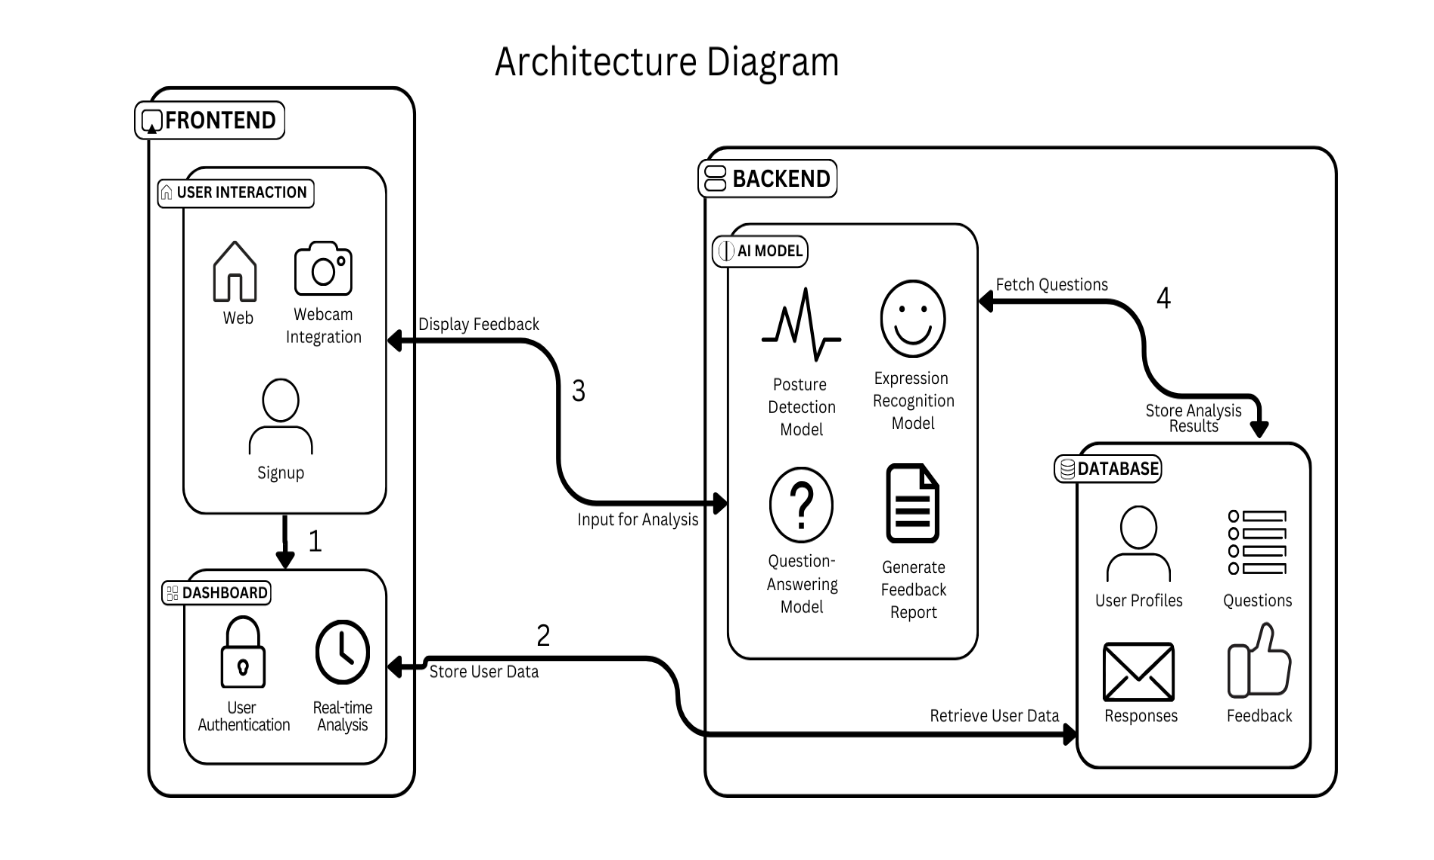
\includegraphics[width=0.8\linewidth]{sections/diagrams/ArchitectureDiagram.png}
\caption{System Architecture Diagram}
\label{fig:architecture}
\end{figure}

\begin{figure}[h]
\centering
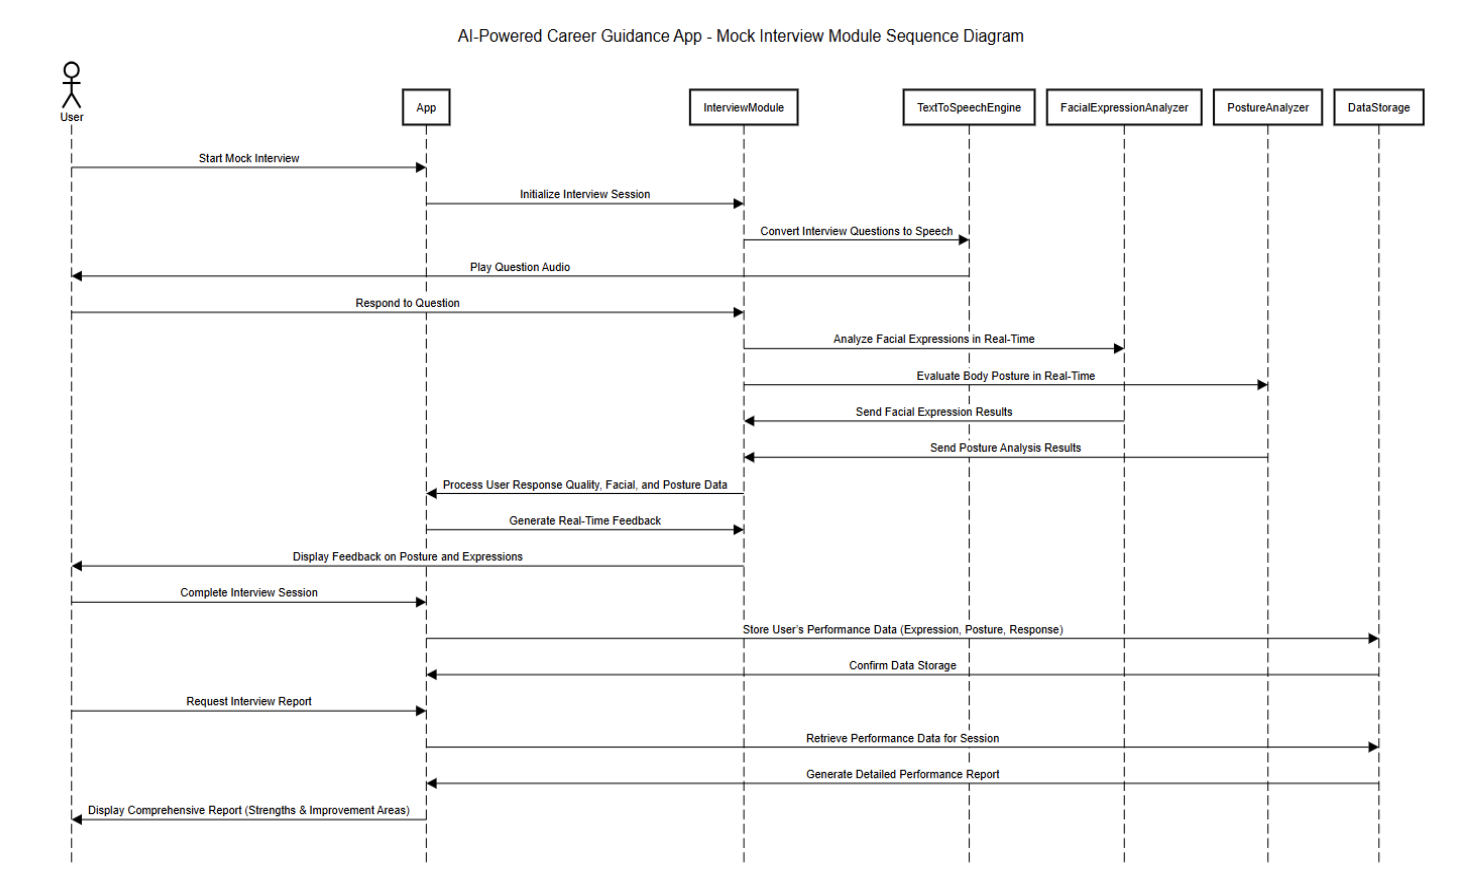
\includegraphics[width=0.8\linewidth]{sections/diagrams/SequentialModel.png}
\caption{Sequential Model Diagram}
\label{fig:sequential}
\end{figure}

\begin{figure}[h]
\centering
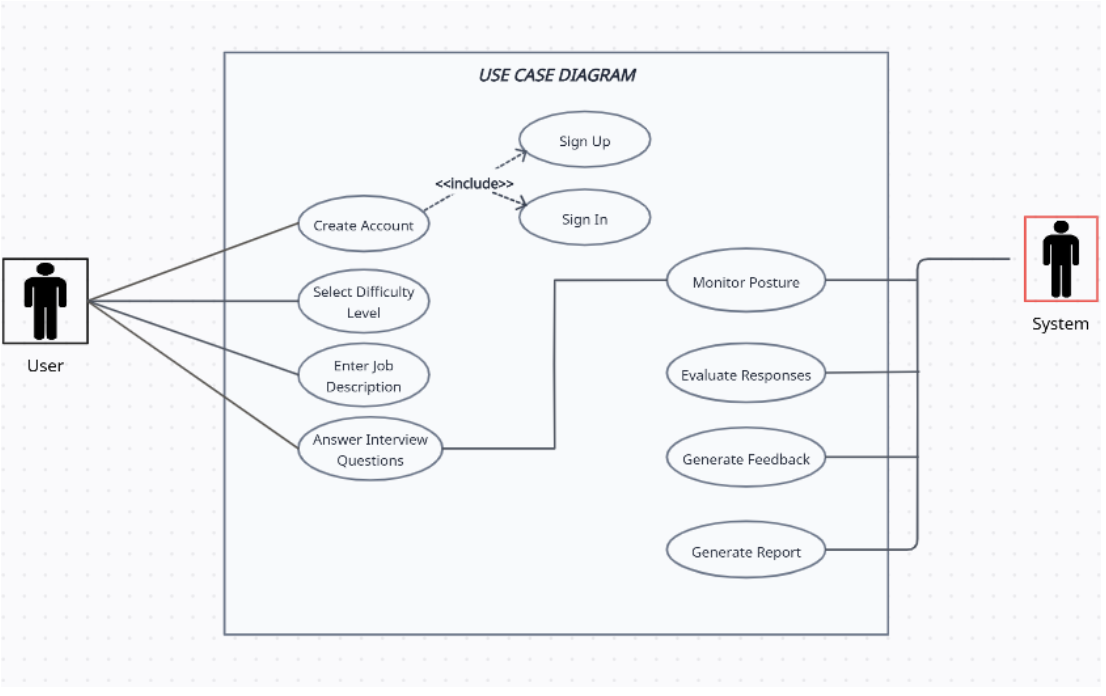
\includegraphics[width=0.8\linewidth]{sections/diagrams/UseCase.png}
\caption{Use Case Diagram}
\label{fig:usecase}
\end{figure}

\begin{figure}[h]
\centering
\begin{tikzpicture}
\begin{umlsystem}[x=4, fill=red!10]{The system}
\umlusecase{Live Interview Analysis}
\umlusecase[y=-2]{Posture Detection}
\umlusecase[y=-4]{Facial Expression Recognition}
\umlusecase[x=4, y=-2, width=1.5cm]{AI Question Generation}
\umlusecase[x=6, fill=green!20]{Interview Scoring}
\umlusecase[x=6, y=-4]{Result Storage}
\end{umlsystem}
\umlactor{User}
\umlactor[y=-3]{Admin}
\umlactor[x=14, y=-1.5]{System}

\umlinherit{Admin}{User}
\umlassoc{User}{usecase-1}
\umlassoc{User}{usecase-2}
\umlassoc{User}{usecase-3}
\umlassoc{System}{usecase-5}
\umlassoc{System}{usecase-6}
\umlinherit{usecase-2}{usecase-1}
\umlVHextend{usecase-5}{usecase-4}
\umlinclude[name=incl]{usecase-3}{usecase-4}
\umlnote[x=7, y=-7]{incl-1}{Real-time AI processing dependency}
\end{tikzpicture}
\caption{Live Interview System Use Case Diagram}
\label{fig:live-interview-usecase}
\end{figure}

---
